\section{Experimentos y Resultados}
% Para la experimentación realizada en este trabajo decidimos comenzar implementando la estrategia \textbf{Grid search},
% la cual nos permitio encontrar la mejor configuracion de hiperparametros entre un subconjunto creado por nosotros. Estos
% hiperparametros son: \textit{learning rate} y \textit{discount} para el algoritmo de \textbf{QLearning}, y el epsilon para
% la politica de control \textbf{$\epsilon-greedy$}. La busqueda fue realizada entre los siguientes valores de cada uno:
%
% \begin{itemize}
%   \item  \textbf{$\epsilon$} = 0.1, 0,2
%   \item \textbf{learning\_rate} = 0.1, 0.2, 0.4, 0.6, 0.8, 0.9, 1.0
%   \item \textbf{discount} = 0.5, 0.6, 0.7, 0.8, 0.9
% \end{itemize}
%
%
% Obteniendo como mejor resultado la siguiente configuracion:
%
% \begin{itemize}
%   \item  \textbf{$\epsilon$} = 0.1
%   \item \textbf{learning\_rate} = 0.4
%   \item \textbf{discount} = 0.9
% \end{itemize}
%
% Ademas de estos hiperparametros para el algoritmo y la politica elegida, tambien necesitamos una cantidad de epocas para
% entrenar y un oponente contra quien jugar.
% Así que tomamos algunas decisiones:

Para la experimentación realizada decidimos utilizar el algoritmo de \textbf{QLearning} para entrenar al agente que jugara
al 4 en linea. Este algoritmo utiliza los hiperparametros \textit{learning rate} y \textit{discount} y la inicializacion
 de la matriz de valores de Q. 
 Ademas de estos hiperparametros, tambien necesitamos una politica de control, una cantidad
  de epocas para entrenar y un oponente contra quien jugar. 

Para este punto notamos que teniamos una explosión combinatoria de parametros, razon por la cual tomamos algunas decisiones
sobre los parametros a utilizar:

\begin{enumerate}
\item La cantidad de epocas para entrenar serán 200.000
\item La política de control que utilizaremos será \textbf{$\epsilon-greedy$}. Y tendremos que elegir el mejor $\epsilon$
\item Nuestro oponente será random.
\item Utilizaremos gridSearch para setear los valores de \textit{learning rate},  \textit{discount} y el valor con que
inicializamos la matriz de Q. Estos tres parametros se moverán entre 0 y 1. Aumentado el valor de a 0.1
\end{enumerate}


El resultado fue que obtuvimos 14641 combinaciones distintas de parametros lo cual fue inviable de probar por cuestiones
 de tiempo. Por este motivo decidimos fijar la inicializacion de la matriz de Q en 0, el \textit{learning rate} y
  \textit{discount} a 0.5, con el objetivo de tomar por igual las recompensas futuras y las actuales, de igual forma
   con la información reciente y la pasada. 

Al fijar estos parametros nos redujo la cantidad de combinaciones posibles a 11. Sin embargo el tiempo que tardaba en entrenar
 seguia siendo muy alto, motivo por el cual se nos ocurrió que en vez de jugar con un tablero de 7x6 y 4 en linea para ganar,
  podíamos acotarlo para ver si se comportaba de modo similar. Tomamos un tablero de 6x5 y 3 en linea para ganar.


%La primer combinacion de parametros tardó aproximadamente 10 min en entrenar. Haciendo una proyeccion de cuanto podria tardar en total con todas las combinaciones tardaria aproximadamente 101 dias, otra señal de que teniamos que reducir la cantidad de combinaciones.

\subsection{Experimento 3 en linea en tablero de $6\times5$}
Para este experimento variamos los diferentes epsilons y obtuvimos que el jugador QLearning ganó el 91\% de las veces con los
siguientes parametros junto con las decisiones tomadas y mencionadas previamente: \\

\begin{itemize}
  \item  \textbf{$\epsilon$} = 0.0
  \item \textbf{learning\_rate} = 0.5
  \item \textbf{discount} = 0.5
  \item \textbf{initialQ} = 0.0
\end{itemize}


%(0.911855, {'discount': 0.5, 'learning_rate': 0.5, 'initialQ': 0.0, 'epsilon': 0.0})

En la siguiente prueba fijamos el valor de $\epsilon$ al mejor resultado 0 y  variamos el learning\_rate del mismo modo.
Obteniendo que con 0.9 ganaba el 95\% de las veces. Luego fijamos learning\_rate a 0.9 e hicimos lo mismo con discount y
gano el 93\% de las veces con 0.1. Es decir que fuimos probando las mejores configuraciones de parametros de forma greedy.

Solo nos restaba variar los valores de inicializacion de matriz Q. Para esto decidimos tomar los mejores resultados del paso
 anterior e inicializarla con valores entre 0 y 1, aumentado en cada paso en 0.1, y tambien probamos que pasaba si
 inicializabamos la matriz con todos los valores random.

El mejor valor obtenido para la inicializacion de Q fue el 0, con el cual nuestro agente gano en el 93\% de las veces.
Por lo tanto, podemos concluir que la mejor combinación que obtuvimos fué:

\begin{itemize}
  \item  \textbf{$\epsilon$} = 0.0
  \item \textbf{learning\_rate} = 0.9
  \item \textbf{discount} = 0.5
  \item \textbf{initialQ} = 0.0
\end{itemize}

Obteniendo los siguientes resultados:

%\begin{frame}
\begin{figure}[h]
 \centering
  \begin{minipage}[c]{1\textwidth}
	\centering
	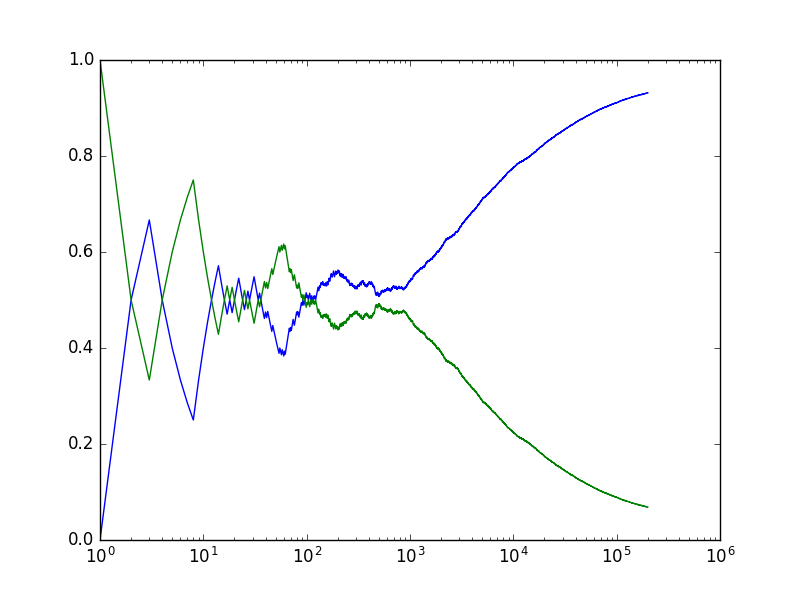
\includegraphics[scale=0.5]{img/QlearningRandomEgreedy200000.png}
        \caption{Qlearning vs Random 200000 juegos}
  \end{minipage}
\end{figure}
%\end{frame}

Lo que podemos observar es que efectivamente el jugador QLearning aprende, pues a medida que aumenta la cantidad de juegos gana mayor cantidad de partidas. Buscamos explicaci\'on y experimentos sobre la aleatoriedad de las victorias en los primeros trials y un por qu\'e gana tanto el jugador Random pero no la encontramos.

Que pasa si jugabamos contra otro jugador Q-learning, bajo la combinación de paramtros obtenida en el paso anterior?.
 Suponemos que en algún momento empezarán a empatar porque ambos aprendieron a jugar.\\

Finalmente, sobre estos parametros podemos concluir que:
\begin{itemize}
  \item  Darle mucho peso a la información reciente da buenos resultados.
  \item  Es tan importante tomar en cuenta las recompesas actuales como las futuras.
  \item  Siempre explotar la informacion que ya conocemos, nunca explorar.
  \item  Es mejor no asignarle ningun valor arbitrario a la matriz de Q. Mejor ir aprendiendo los valores en funcion de
   los juegos.
\end{itemize}

%%%%%%%%%%%%%%%%%%%%%%%

Luego de realizados estos experimentos, decidimos variar la cantidad de epocas para el caso donde juegan dos Qlearners,
obteniendo los siguientes resultados:

\begin{figure}[h]
 \centering
 \begin{minipage}{.45\textwidth}
  %\begin{minipage}[c]{1\textwidth}
	\centering
	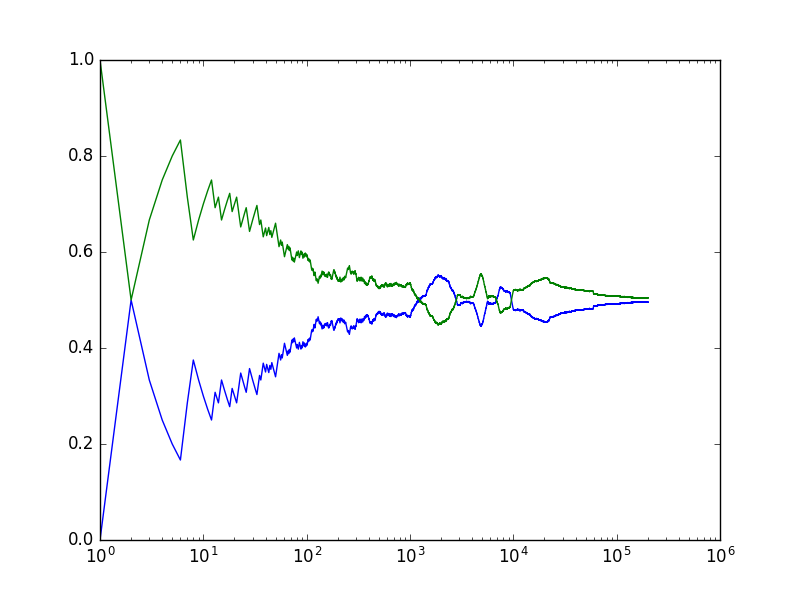
\includegraphics[scale=0.35]{img/QlearningQlearningEgreedy200000.png}
        \caption{QL vs QL 200000 juegos}
  \end{minipage}
 \begin{minipage}{.5\textwidth}
	\centering
	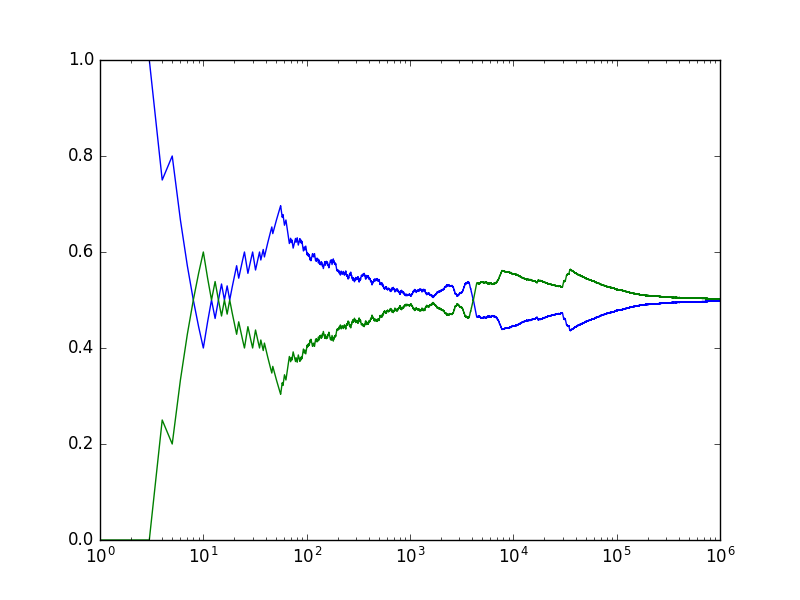
\includegraphics[scale=0.35]{img/QlearningQlearningEgreedy1000000.png}
        \caption{QL vs QL 1000000 juegos}
  \end{minipage}
\end{figure}

\begin{figure}[h]
 \centering
 \begin{minipage}{.45\textwidth}
  %\begin{minipage}[c]{1\textwidth}
	\centering
	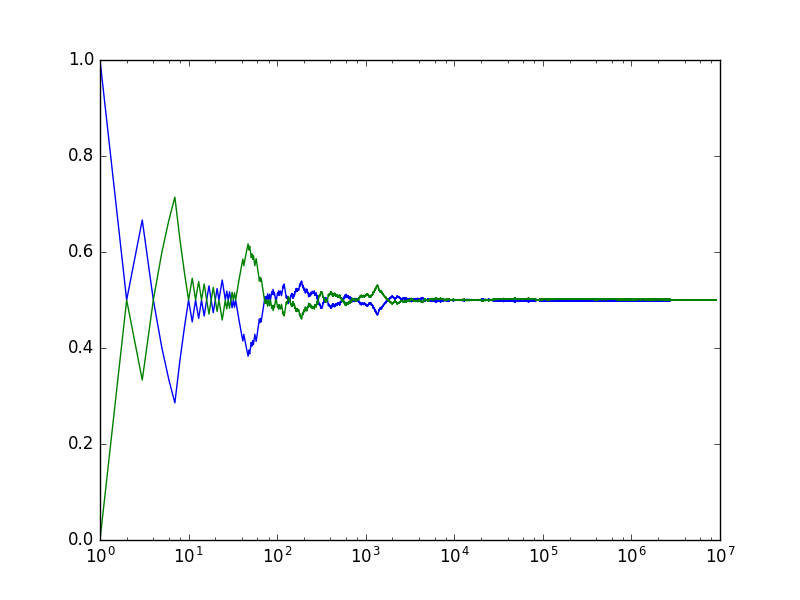
\includegraphics[scale=0.35]{img/QlearningQlearningEgreedy9000000.png}
        \caption{QL vs QL 9000000 juegos}
  \end{minipage}
\end{figure}

Podemos ver como a la hora de enfrentarse contra otro jugador, que tambien aprende, llega un momento donde se estabiliza la
 cantidad de veces que gana cada uno. Esto no se corresponde con la idea que teniamos. 

Asi que decidimos jugar contra el jugador Q-learning entrenado para ver c\'omo estaba jugando. Y lo que notamos es que siempre que el primer turno sea de \'el, utilizaba una estrategia ganadora. Tambi\'en se defend\'ia bien cuando era su turno, es decir, no aprendi\'o algo en detrimento de lo otro.

La estregia es muy parecida a la de que se utiliza en el juego de ta-te-ti de formar una L, hace una serie de movimientos que lleva a que el contrincante sin importar donde ponga la pr\'oxima ficha, el Qlearner tiene otras dos posibilidades para ganar. Para que el lector pueda probar esto y jugar, se puede cargar el modelo desde la l\'inea de comando.

Nos pareci\'o muy llamativa este comportamiento que logr\'o el Qlearner, y lo tomamos como una prueba fehaciente que el modelo realmente est\'a aprendiendo la naturaleza detr\'as del juego. Mientras que una persona tardar\'ia bastante tiempo en encontrar la estrategia ganadora, el algoritmo lo encontr\'o simplemente al jugar repetidas veces contra un jugador que tira acciones random.

Y esto explicaría por que no empatan. Como el jugador que comienza tiene una estrategia ganadora siempre va a ganar.\\

Sin embargo estamos jugando un juego con un tablero de dimension menor, asi que queremos ver que pasa si entrenamos
 con los mismos parametros y las caracteristicas del juego original.

\subsection{Experimento 4 en linea en tablero de $7\times6$}
En esta seccion experimentamos con el tablero original de $7\times6$, y las reglas originales del 4 en linea, obteniendo
los siguientes resultados:

\begin{figure}[h]
 \centering
  \begin{minipage}[c]{1\textwidth}
	\centering
	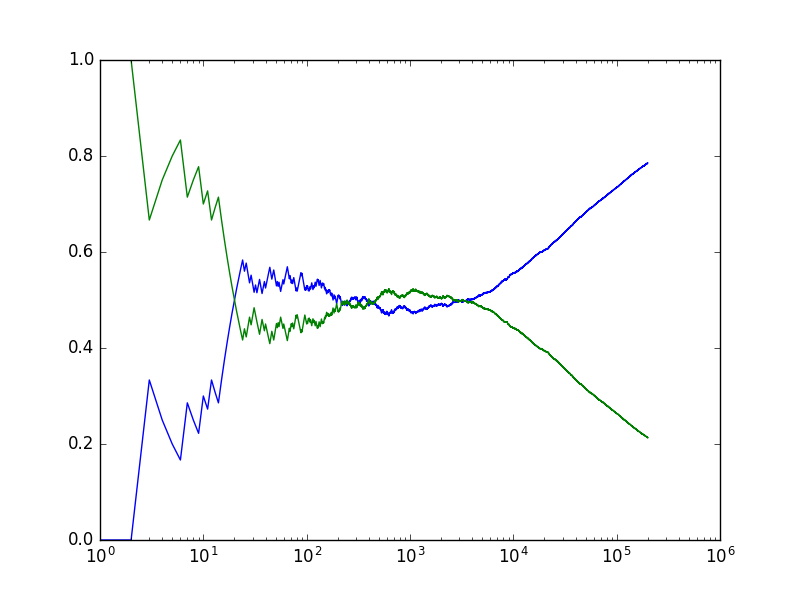
\includegraphics[scale=0.5]{img/QlearningRandomEgreedy2000007x6(4).png}
        \caption{QL vs Random 200000 juegos}
  \end{minipage}
\end{figure}

Lo que podemos observar es bastante razonable, como agrandamos el tablero tenemos muchas mas combinaciones, motivo por el cual,
 tarda mas tiempo en aprender como ganar.

En este caso ya no encontramos estrategia ganadora para los mismos parametros.
{\huge EXPLICAR MEJOR ESTO}\\


\begin{figure}[h]
 \centering
 \begin{minipage}{.45\textwidth}
	\centering
	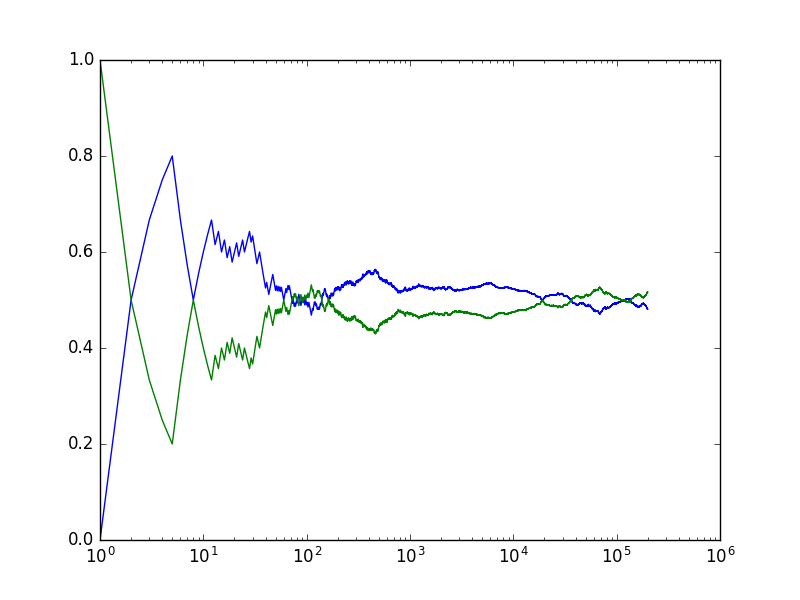
\includegraphics[scale=0.35]{img/QlearningQlearningEgreedy2000007x6(4).png}
       \caption{QL vs QL 200000 juegos}
  \end{minipage}
% \begin{minipage}{.5\textwidth}
%	\centering
%	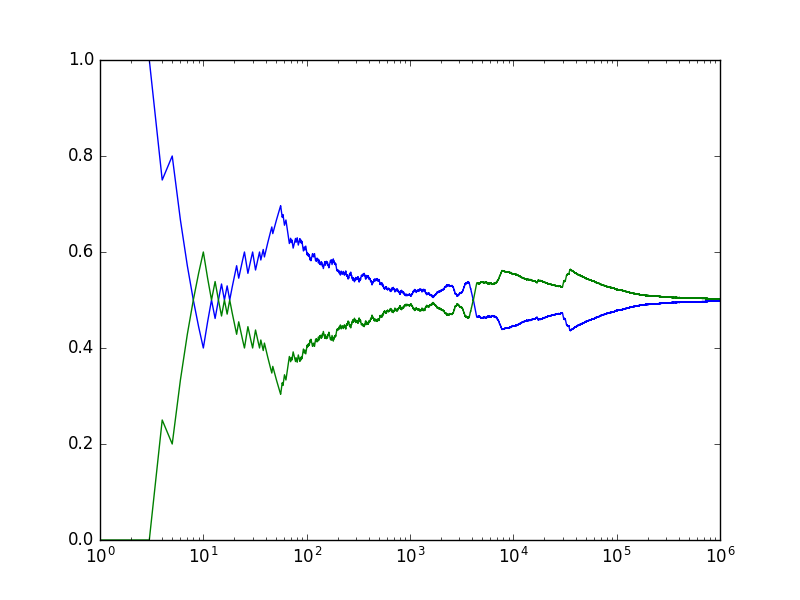
\includegraphics[scale=0.35]{img/QlearningQlearningEgreedy1000000.png}
%        \caption{Qlearning vs Qlearning 1000000 juegos}
%  \end{minipage}
\end{figure}

No pudimos probar Qlearning Vs Qlearning con 9000000 juegos debido al tiempo de computo.


Asi que pensamos en probar otra politica de control softmax.

Otra vez nos dimos a la tarea de buscar los parametros. En este caso necesitamos definir un tau y una funcion de decremento
 ademas de textit{learning rate}, \textit{discount}, cantidad de epocas, y los valores de inicializacion de Q. Para estos ultimos exploramos valores que se encontraban alrededor de los encontrados para la estrategia e-greedy.
Empezamos con el tabler de 6x5 y 3 fichas y una vez encontrado los parametros pasamos al tablero real.






%
% \subsection{Experimento 4 en linea en tablero de $7\times6$}
% En el siguiente experimento decidimos entrenar con el juego completo de 4 en linea, en su formato original de un tablero
% de $7\times6$. Para este caso decidimos experimentar con dos politicas de control: \textit{$\epsilon-greedy$} y
% \textit{softmax}. En ambos casos realizamos 500000 iteraciones de juego, y para cada caso entrenamos a nuestro agente
% contra un jugador random y contra otro agente de Qlearning. \\
% Los parametros utilizados tanto para \textit{$\epsilon-greedy$}, como para \textit{softmax} fueron los obtenidos por la
% estrategia de Grid search previamente explicada.
%
% Los resultados obtenidos en cada caso fueron:
%
% \todo{Poner resultados Qlearn vs Qlearn(epsilon greedy)}
%
% \todo{Poner resultados Qlearn vs Qlearn(softmax)}
%
% \todo{Poner resultados Qlearn vs random(epsilon greedy)}
%
% \todo{Poner resultados Qlearn vs random(softmax)}
%
% \subsection{Experimento 3 en linea en tablero de $6\times5$}
